\subsection{Die Ratiaonalen Zahlen}
Symbol: $\mathbb{Q}$\\
sind die Menge aller Brüche

\hfill \break
\hfill \break
$ \mathbb{Q}=\{\frac{2}{3},\frac{7}{6},\frac{1}{6},1\frac{6}{7},0.125,0.\overline{3},\ldots\} $

\hfill \break
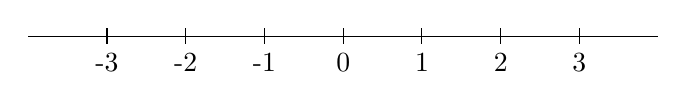
\begin{tikzpicture}
    \draw (-4,0) -- (4,0);
    \foreach \X in {-3,...,3}
    \draw (\X,0.1) -- (\X,-0.1);
    \foreach \X in {-3,-2,-1,0,1,2,3}
    \node[anchor=north] at (\X,-0.1){\X};
\end{tikzpicture}

\hfill \break
Benennung: 1/3 = $\frac{1}{3} = 0.\overline{3}$
\begin{itemize}
    \item 1 = Zähler, er zählt wie oft die Basis vorhanden ist
    \item 3 = Nenner, er gibt die Basis an
\end{itemize}

\hfill \break
Es bibt endliche und unendliche Dezimalzahlen:
\begin{itemize}
    \item endliche: 0.25
    \item unendliche: $0.\overline{25}$
\end{itemize}

\hfill \break
Möglichkeiten mit den Ganzen Zahlen:
\begin{enumerate}
    \item Dividieren ist ist uneingeschränkt möglich:
          \begin{itemize}
              \item 1/3 = $0.\overline{3}$
              \item 10/5 = 2
          \end{itemize}
\end{enumerate}

\hfill \break
Bekannte Büche:
\begin{itemize}
    \item $\frac{1}{5} = 0.2$
    \item $\frac{1}{4} = 0.25$
    \item $\frac{1}{2} = 0.5$
    \item $\frac{1}{8} = 0.125$
    \item $\frac{1}{9} = 0.\overline{1}$
    \item $\frac{1}{3} = 0.\overline{3}$
\end{itemize}